\section{Derivation of the Wiener response}
\label{app:wiener}

We expand the linear-MMSE argument of Sec.~\ref{sec:gate}. Work in one
channel and assume wide-sense stationarity, so that convolution
diagonalizes in the Fourier basis and the mean-square error splits per
frequency.

\paragraph{Setup.} Under the mixture $x_t = a_t x_0 + b_t \varepsilon$ with
$\varepsilon$ white and independent of $x_0$, let $S_x(f)$ be the power
spectrum of $x_0$. For a linear filter $h_t$ with response $H_t(f)$,
Parseval's identity gives
\begin{equation}
  J_t(h_t) = \sum_f \Big(
  |H_t(f)|^2\big(a_t^2 S_x(f) + b_t^2\big)
  - 2\,\mathrm{Re}\big[H_t(f)\,a_t S_x(f)\big]
  + S_x(f)\Big).
  \label{eq:app-mse}
\end{equation}

\paragraph{Optimality by differentiation.} The summands decouple, so each
$H_t(f)$ solves a scalar problem. Differentiating with respect to
$\overline{H_t(f)}$ and setting to zero,
\begin{equation}
  H_t(f)\big(a_t^2 S_x(f) + b_t^2\big) - a_t S_x(f) = 0,
\end{equation}
which yields~\eqref{eq:wiener}. The second derivative
$a_t^2 S_x(f) + b_t^2 > 0$ confirms a minimum.

\paragraph{Power-law prior and spectral evolution.}
Natural images obey $S_x(f) \propto 1/|f|^p$ with $p \approx 2$.
Inserting this into~\eqref{eq:wiener}: at large $t$ (small $a_t$) the
denominator is noise-dominated except near $f = 0$, so $G_t$ is low-pass;
as $t \to 0$ ($a_t \to 1$) the passband widens toward high frequencies.
Fig.~\ref{fig:app-filters} plots the exact responses along the flow
schedule. This is the spectral evolution tracked by the filtered
distance of Sec.~\ref{sec:gate}, and the mean-gain
normalization~\eqref{eq:norm} makes those distances comparable across
$t$: the raw gains in Fig.~\ref{fig:app-filters}(a) differ by orders of
magnitude across $\sigma$, whereas the normalized responses in (b) share
a common scale and differ only in shape.

\begin{figure}[h]
  \centering
  
\includegraphics[width=0.95\linewidth]{figA_filters.pdf}
  \caption{Wiener filter responses along the flow schedule
  ($a_t = 1-\sigma$, $b_t = \sigma$, $S_x(f) = 1/|f|^p$, $p{=}2$ as used
  for FLUX; the video models use $p{=}3$ with the same qualitative
  shape). The formula is identical to SeaCache's; only the plotted
  schedule instance differs (flow, as used by our gate, vs.\ their
  DPM illustration). (a)~Raw response $G_t(f)$: low-pass early (large
  $\sigma$), widening as $\sigma \to 0$. (b)~Mean-normalized
  $G_t^{\mathrm{norm}}(f)$: comparable energy across timesteps, so
  accumulated distances are not dominated by gain drift. Computed from
  the closed form of~\eqref{eq:wiener}.}
  \label{fig:app-filters}
\end{figure}

%----------------------------------------------------------------

\begingroup
\color{red}
\section{Approximation Bounds for the Predictors}
\label{app:predictor-bounds}

This appendix establishes the approximation bounds used in
Sec.~\ref{sec:hierarchy}. The analysis is channel-wise. Throughout,
$t_k$ denotes the most recent evaluated step, $t_j$ denotes the skipped
step at which the residual is reconstructed, and
\[
\ell_{jk}:=|t_j-t_k|
\]
denotes the current skip length.

\paragraph{Copy-reuse.}
Copy-reuse sets
\[
\widehat r_{\mathrm{copy}}(t_j)=r(t_k).
\]
If $r$ is $L_r$-Lipschitz on an interval containing $t_k$ and $t_j$,
then
\begin{equation}
\left|
r(t_j)-\widehat r_{\mathrm{copy}}(t_j)
\right|
=
|r(t_j)-r(t_k)|
\leq
L_r\ell_{jk}.
\label{eq:app-copy-bound}
\end{equation}
The bound is sharp over the class of $L_r$-Lipschitz functions, since
$r(t)=L_rt$ attains equality.

\paragraph{Ideal Taylor extrapolation.}
Suppose that $r\in C^{P+1}(I)$ on a closed interval $I$ containing
$t_k$ and $t_j$. Taylor's theorem gives
\begin{equation}
r(t_j)
=
\sum_{p=0}^{P}
\frac{r^{(p)}(t_k)}{p!}
(t_j-t_k)^p
+
\frac{r^{(P+1)}(\xi)}{(P+1)!}
(t_j-t_k)^{P+1},
\label{eq:app-taylor-expansion}
\end{equation}
where $\xi$ lies between $t_k$ and $t_j$. Hence,
\begin{equation}
\left|
r(t_j)
-
\sum_{p=0}^{P}
\frac{r^{(p)}(t_k)}{p!}
(t_j-t_k)^p
\right|
\leq
\frac{
\|r^{(P+1)}\|_{\infty,I}
}{
(P+1)!
}
\ell_{jk}^{P+1}.
\label{eq:app-taylor-bound}
\end{equation}
This estimate is an oracle reference rate because the proposed
procedure does not compute the exact derivatives $r^{(p)}(t_k)$.

\paragraph{Discrete polynomial extrapolation.}
Let $s_0,\ldots,s_P$ be $P+1$ distinct evaluated nodes, with
$s_0=t_k$, and let $p_P$ be the degree-$P$ interpolating polynomial
satisfying
\[
p_P(s_q)=r(s_q),
\qquad
q=0,\ldots,P.
\]
Assume that $r\in C^{P+1}(I)$ on a closed interval $I$ containing
$t_j,s_0,\ldots,s_P$. The interpolation remainder gives
\begin{equation}
r(t_j)-p_P(t_j)
=
\frac{r^{(P+1)}(\xi)}{(P+1)!}
\prod_{q=0}^{P}(t_j-s_q)
\label{eq:app-interpolation-remainder}
\end{equation}
for some $\xi$ in the convex hull of
$\{t_j,s_0,\ldots,s_P\}$. Therefore,
\begin{equation}
|r(t_j)-p_P(t_j)|
\leq
\frac{
\|r^{(P+1)}\|_{\infty,I}
}{
(P+1)!
}
\prod_{q=0}^{P}|t_j-s_q|.
\label{eq:app-interpolation-bound}
\end{equation}

The product in~\eqref{eq:app-interpolation-bound} cannot generally be
replaced by a node-independent multiple of $\ell_{jk}^{P+1}$. Consider
\[
P=1,
\qquad
r(t)=t^2,
\qquad
s_0=t_k=0,
\qquad
s_1=-H,
\qquad
t_j=\ell,
\]
where $H>0$ and $\ell>0$. The linear interpolant is
\[
p_1(t)=-Ht.
\]
Consequently,
\begin{equation}
|r(\ell)-p_1(\ell)|
=
\ell(\ell+H),
\end{equation}
and
\begin{equation}
\frac{|r(\ell)-p_1(\ell)|}{\ell^2}
=
1+\frac{H}{\ell}.
\label{eq:app-counterexample-ratio}
\end{equation}
This ratio is unbounded as $H/\ell\to\infty$. Therefore, no constant
independent of the evaluated-node locations can yield a bound of the
form
\[
|r(t_j)-p_P(t_j)|
\leq
C\ell_{jk}^{P+1}
\]
for arbitrary evaluated nodes.

For uniformly spaced backward nodes
\[
t_j=t_k+\ell_{jk},
\qquad
s_q=t_k-qh,
\qquad
h>0,
\]
the correct product is
\begin{equation}
\prod_{q=0}^{P}|t_j-s_q|
=
\prod_{q=0}^{P}(\ell_{jk}+qh).
\label{eq:app-uniform-product}
\end{equation}
Although this is a degree-$(P+1)$ polynomial in $\ell_{jk}$, it is not
equal to $\ell_{jk}^{P+1}$ at finite $\ell_{jk}$. Uniform spacing alone
therefore does not recover the ideal Taylor remainder.

If
\begin{equation}
\max_{0\leq q\leq P}|t_j-s_q|
\leq
C_{\mathrm{node}}\ell_{jk},
\end{equation}
then
\begin{equation}
|r(t_j)-p_P(t_j)|
\leq
\frac{
C_{\mathrm{node}}^{P+1}
\|r^{(P+1)}\|_{\infty,I}
}{
(P+1)!
}
\ell_{jk}^{P+1}.
\end{equation}
Thus, an order-$(P+1)$ skip-length estimate for the discrete predictor
requires control of the preceding node positions relative to the current
forecast distance.

\paragraph{Chebyshev truncation.}
Map the solver index affinely to $\tau\in[-1,1]$. Suppose that $r$
extends analytically to the Bernstein ellipse $E_\rho$, where
$\rho>1$, and satisfies
\[
\sup_{z\in E_\rho}|r(z)|\leq B.
\]
Let
\[
p_M^\star(\tau)
=
\sum_{m=0}^{M}c_m^\star T_m(\tau)
\]
be its degree-$M$ Chebyshev truncation. The coefficients satisfy
\[
|c_0^\star|\leq B,
\qquad
|c_m^\star|\leq2B\rho^{-m},
\quad m\geq1.
\]
Because $|T_m(\tau)|\leq1$ on $[-1,1]$,
\begin{align}
\|r-p_M^\star\|_\infty
&\leq
\sum_{m=M+1}^{\infty}|c_m^\star|
\nonumber\\
&\leq
\sum_{m=M+1}^{\infty}2B\rho^{-m}
\nonumber\\
&=
\frac{2B}{\rho-1}\rho^{-M}
=:
\varepsilon_M.
\label{eq:app-chebyshev-bound}
\end{align}
This truncation bound is uniform in the evaluation point and contains no
explicit dependence on the current skip length. It does not, by itself,
bound the complete fitted forecast error. The additional finite-history
and ridge-shrinkage terms depend on the realized Chebyshev design
matrix, as quantified in Lemma~\ref{lem:ridge}.

\paragraph{Node spacing and design conditioning.}
The relative node-spacing condition in
\eqref{eq:relative-node-spacing} and the design-conditioning quantity
$\sigma_{\min}(\mathbf{\Phi}_n)$ in Lemma~\ref{lem:ridge} are distinct
properties of the realized evaluation schedule. The former controls the
local interpolation remainder, whereas the latter controls the
stability of the fitted Chebyshev coefficients. Neither condition
implies the other.

For the first direction, suppose
\[
t_j=t_k+\ell_{jk},
\qquad
s_q=t_k-\delta_q,
\qquad
\delta_q\geq0,
\qquad
\max_q\delta_q\longrightarrow0,
\]
while $\ell_{jk}>0$ remains fixed. Then
\begin{equation}
\frac{
\max_q|t_j-s_q|
}{
\ell_{jk}
}
=
1+
\frac{\max_q\delta_q}{\ell_{jk}}
\longrightarrow1.
\end{equation}
Thus, the relative node-spacing condition holds uniformly, with
$C_{\mathrm{node}}\to1$. Under the fixed affine normalization used to
form the Chebyshev design, however, the rows of $\mathbf{\Phi}_n$
become nearly identical. For a nonconstant polynomial basis,
\begin{equation}
\sigma_{\min}(\mathbf{\Phi}_n)\longrightarrow0
\end{equation}
as the nodes coalesce.

Conversely, consider $P=1$, $s_0=t_k=0$, and $s_1=-H_0$ for a fixed
$H_0>0$. Since these interpolation nodes do not depend on the forecast
distance $\ell$, the matrix
\[
\mathbf{\Phi}
=
\begin{bmatrix}
1 & 0\\
1 & -H_0
\end{bmatrix}
\]
is fixed and nonsingular. Its conditioning therefore remains fixed as
$\ell$ varies. If $t_j=\ell>0$, then
\begin{equation}
\frac{
\max_{q\in\{0,1\}}|t_j-s_q|
}{
|t_j-t_k|
}
=
\frac{\ell+H_0}{\ell}
\longrightarrow\infty
\qquad
\text{as }\ell\to0^+.
\end{equation}
Thus, the design conditioning remains fixed while no uniform finite
relative node-spacing constant exists over this family.

The copy-reuse, ideal Taylor, local interpolation, and Chebyshev bounds
apply under different regularity and sampling assumptions. They
identify distinct error mechanisms, but they do not establish a strict
ordering of the actual forecast errors over a common function class.

\endgroup


\begingroup
\color{red}

\section{Proof of Lemma~\ref{lem:ridge} (ridge stability)}
\label{app:ridge}

Fix one residual channel and suppress the channel index. Let
\[
\mathbf{y}
=
\mathbf{\Phi}_n\mathbf{c}^\star+\mathbf{e},
\]
where
\[
\mathbf{\Phi}_n\in\mathbb{R}^{n\times(M+1)}
\]
is the Chebyshev design matrix associated with the currently observed
nodes $\tau_1,\ldots,\tau_n$, and $\mathbf{c}^\star$ is the coefficient
vector of the exact degree-$M$ Chebyshev truncation $p_M^\star$.
By~\eqref{eq:cheb},
\[
|e_k|
=
|r(\tau_k)-p_M^\star(\tau_k)|
\leq
\varepsilon_M,
\qquad
k=1,\ldots,n.
\]
Therefore,
\begin{equation}
\|\mathbf{e}\|_2
\leq
\sqrt{n}\,\varepsilon_M.
\label{eq:app-error-vector}
\end{equation}

For $\lambda>0$, define
\[
A_\lambda
=
\mathbf{\Phi}_n^\top\mathbf{\Phi}_n+\lambda I.
\]
The ridge estimator is
\[
\widehat{\mathbf{c}}
=
A_\lambda^{-1}\mathbf{\Phi}_n^\top\mathbf{y}.
\]
Consequently,
\begin{align}
\widehat{\mathbf{c}}-\mathbf{c}^\star
&=
A_\lambda^{-1}\mathbf{\Phi}_n^\top
\left(
\mathbf{\Phi}_n\mathbf{c}^\star+\mathbf{e}
\right)
-\mathbf{c}^\star
\nonumber\\
&=
A_\lambda^{-1}
\mathbf{\Phi}_n^\top\mathbf{\Phi}_n\mathbf{c}^\star
-\mathbf{c}^\star
+
A_\lambda^{-1}\mathbf{\Phi}_n^\top\mathbf{e}
\nonumber\\
&=
A_\lambda^{-1}
\left(
A_\lambda-\lambda I
\right)
\mathbf{c}^\star
-\mathbf{c}^\star
+
A_\lambda^{-1}\mathbf{\Phi}_n^\top\mathbf{e}
\nonumber\\
&=
A_\lambda^{-1}\mathbf{\Phi}_n^\top\mathbf{e}
-
\lambda A_\lambda^{-1}\mathbf{c}^\star.
\label{eq:app-split}
\end{align}

\paragraph{Propagation of the truncation residual.}
Define
\[
\sigma_{\min}
=
\sqrt{
\lambda_{\min}
\left(
\mathbf{\Phi}_n^\top\mathbf{\Phi}_n
\right)
},
\qquad
\sigma_{\max}
=
\|\mathbf{\Phi}_n\|_2.
\]
Here $\sigma_{\min}=0$ whenever $\mathbf{\Phi}_n$ is rank deficient;
equivalently, zero singular values are included in this definition.

Using the singular-value decomposition of $\mathbf{\Phi}_n$, we obtain
\begin{align}
\left\|
A_\lambda^{-1}\mathbf{\Phi}_n^\top
\right\|_2
&=
\max_i
\frac{
\sigma_i(\mathbf{\Phi}_n)
}{
\sigma_i^2(\mathbf{\Phi}_n)+\lambda
}
\nonumber\\
&\leq
\frac{
\sigma_{\max}
}{
\sigma_{\min}^2+\lambda
}.
\label{eq:app-ridge-operator}
\end{align}
Combining~\eqref{eq:app-error-vector} and
\eqref{eq:app-ridge-operator} gives
\begin{align}
\left\|
A_\lambda^{-1}\mathbf{\Phi}_n^\top\mathbf{e}
\right\|_2
&\leq
\left\|
A_\lambda^{-1}\mathbf{\Phi}_n^\top
\right\|_2
\|\mathbf{e}\|_2
\nonumber\\
&\leq
\frac{
\sigma_{\max}\sqrt{n}
}{
\sigma_{\min}^2+\lambda
}
\,\varepsilon_M.
\label{eq:app-truncation-term}
\end{align}

\paragraph{Ridge-shrinkage bias.}
Analyticity in the Bernstein ellipse $E_\rho$ and the bound
\[
\sup_{z\in E_\rho}|r(z)|\leq B
\]
imply
\[
|c_0^\star|\leq B,
\qquad
|c_m^\star|\leq2B\rho^{-m},
\quad m\geq1.
\]
Hence,
\begin{align}
\|\mathbf{c}^\star\|_2^2
&\leq
B^2+
4B^2\sum_{m=1}^{M}\rho^{-2m}
\nonumber\\
&\leq
B^2+
4B^2\sum_{m=1}^{\infty}\rho^{-2m}
\nonumber\\
&=
B^2+
\frac{4B^2\rho^{-2}}{1-\rho^{-2}}
\nonumber\\
&\leq
\frac{4B^2}{1-\rho^{-2}}.
\end{align}
Therefore,
\begin{equation}
\|\mathbf{c}^\star\|_2
\leq
\frac{2B}{\sqrt{1-\rho^{-2}}}.
\label{eq:app-coefficient-bound}
\end{equation}

By the definition of $\sigma_{\min}$,
\[
\|A_\lambda^{-1}\|_2
=
\frac{1}{\sigma_{\min}^2+\lambda}.
\]
Thus,
\begin{align}
\left\|
\lambda A_\lambda^{-1}\mathbf{c}^\star
\right\|_2
&\leq
\lambda
\|A_\lambda^{-1}\|_2
\|\mathbf{c}^\star\|_2
\nonumber\\
&\leq
\frac{
2B\lambda
}{
\bigl(\sigma_{\min}^2+\lambda\bigr)
\sqrt{1-\rho^{-2}}
}.
\label{eq:app-bias-term}
\end{align}

\paragraph{Evaluation at the forecast point.}
Let
\[
\boldsymbol{\phi}(\tau_j)
=
\bigl(
T_0(\tau_j),\ldots,T_M(\tau_j)
\bigr)^\top.
\]
Because $\tau_j\in[-1,1]$ and $|T_m(\tau_j)|\leq1$,
\[
\|\boldsymbol{\phi}(\tau_j)\|_2
\leq
\sqrt{M+1}.
\]
Moreover,
\[
\widehat r(\tau_j)
=
\boldsymbol{\phi}(\tau_j)^\top\widehat{\mathbf{c}},
\qquad
p_M^\star(\tau_j)
=
\boldsymbol{\phi}(\tau_j)^\top\mathbf{c}^\star.
\]
Therefore,
\begin{align}
\left|
\widehat r(\tau_j)-p_M^\star(\tau_j)
\right|
&=
\left|
\boldsymbol{\phi}(\tau_j)^\top
\left(
\widehat{\mathbf{c}}-\mathbf{c}^\star
\right)
\right|
\nonumber\\
&\leq
\|\boldsymbol{\phi}(\tau_j)\|_2
\left\|
\widehat{\mathbf{c}}-\mathbf{c}^\star
\right\|_2
\nonumber\\
&\leq
\frac{
\sigma_{\max}\sqrt{n(M+1)}
}{
\sigma_{\min}^2+\lambda
}
\,\varepsilon_M
\nonumber\\
&\quad+
\frac{
2B\lambda\sqrt{M+1}
}{
\bigl(\sigma_{\min}^2+\lambda\bigr)
\sqrt{1-\rho^{-2}}
}.
\end{align}
This proves~\eqref{eq:ridge-stability}.

Finally, by the triangle inequality and the uniform Chebyshev
truncation estimate,
\begin{align}
\left|
\widehat r(\tau_j)-r(\tau_j)
\right|
&\leq
\left|
\widehat r(\tau_j)-p_M^\star(\tau_j)
\right|
+
\left|
p_M^\star(\tau_j)-r(\tau_j)
\right|
\nonumber\\
&\leq
\varepsilon_M
+
\frac{
\sigma_{\max}\sqrt{n(M+1)}
}{
\sigma_{\min}^2+\lambda
}
\,\varepsilon_M
\nonumber\\
&\quad+
\frac{
2B\lambda\sqrt{M+1}
}{
\bigl(\sigma_{\min}^2+\lambda\bigr)
\sqrt{1-\rho^{-2}}
}.
\end{align}
This proves~\eqref{eq:complete-forecast-bound}.

\endgroup

%----------------------------------------------------------------
\section{Residual-Space Error Identity and Target Scaling}
\label{app:residual}

In this section,
$\mathbf{h}_{\mathrm{in}}(t)$ and
$\mathbf{h}_{\mathrm{out}}(t)$ denote the input and output of the entire
cached transformer segment. In particular,
$\mathbf{h}_{\mathrm{in}}(t)$ is available before that segment is
evaluated. Define the transformer residual by
\begin{equation}
\mathbf{r}(t)
=
\mathbf{h}_{\mathrm{out}}(t)
-
\mathbf{h}_{\mathrm{in}}(t).
\label{eq:residual-definition}
\end{equation}

\paragraph{Skipped-step error identity.}
If a skipped output is reconstructed from a residual forecast as
\begin{equation}
\widehat{\mathbf{h}}_{\mathrm{out}}(t_j)
=
\mathbf{h}_{\mathrm{in}}(t_j)
+
\widehat{\mathbf{r}}(t_j),
\label{eq:residual-reconstruction}
\end{equation}
then
\begin{align}
\widehat{\mathbf{h}}_{\mathrm{out}}(t_j)
-
\mathbf{h}_{\mathrm{out}}(t_j)
&=
\mathbf{h}_{\mathrm{in}}(t_j)
+
\widehat{\mathbf{r}}(t_j)
-
\left(
\mathbf{h}_{\mathrm{in}}(t_j)
+
\mathbf{r}(t_j)
\right)
\nonumber\\
&=
\widehat{\mathbf{r}}(t_j)
-
\mathbf{r}(t_j).
\label{eq:residual-error-identity}
\end{align}
Thus, when a skipped output is reconstructed from a given residual
forecast, its reconstruction error is exactly the residual-forecast
error.

\paragraph{Trajectory matrices.}
Suppose that residuals have been observed at
$t_1,\ldots,t_n$. Stack the corresponding feature vectors row-wise:
\begin{align}
\mathbf{H}_{\mathrm{in}}
&=
\begin{bmatrix}
\mathbf{h}_{\mathrm{in}}(t_1)^\top\\
\vdots\\
\mathbf{h}_{\mathrm{in}}(t_n)^\top
\end{bmatrix}
\in\mathbb{R}^{n\times F},
\\
\mathbf{H}_{\mathrm{out}}
&=
\begin{bmatrix}
\mathbf{h}_{\mathrm{out}}(t_1)^\top\\
\vdots\\
\mathbf{h}_{\mathrm{out}}(t_n)^\top
\end{bmatrix}
\in\mathbb{R}^{n\times F},
\\
\mathbf{R}
&=
\begin{bmatrix}
\mathbf{r}(t_1)^\top\\
\vdots\\
\mathbf{r}(t_n)^\top
\end{bmatrix}
\in\mathbb{R}^{n\times F}.
\end{align}
The correct matrix identity is
\begin{equation}
\mathbf{H}_{\mathrm{out}}
=
\mathbf{H}_{\mathrm{in}}
+
\mathbf{R}.
\label{eq:state-residual-matrix}
\end{equation}
In general, $\mathbf{H}_{\mathrm{in}}$ varies with the sampling step
and is not rank one. Therefore, we do not assume a decomposition of the
form
$\mathbf{h}_{\mathrm{in}}\mathbf{1}^\top+\mathbf{R}$.

\paragraph{Common design conditioning.}
Let
\begin{equation}
\mathbf{\Phi}_n\in\mathbb{R}^{n\times d}
\end{equation}
be the Chebyshev design matrix, where $d$ is the number of retained
basis functions. Under the degree-$M$ convention
$T_0,\ldots,T_M$, one has $d=M+1$. Define
\begin{equation}
\mathbf{A}_\lambda
=
\mathbf{\Phi}_n^\top\mathbf{\Phi}_n+\lambda I_d,
\qquad
\lambda>0.
\label{eq:residual-ridge-matrix}
\end{equation}
For an arbitrary target matrix
$\mathbf{Y}\in\mathbb{R}^{n\times F}$, define its ridge coefficient
estimate by
\begin{equation}
\widehat{\mathbf{C}}(\mathbf{Y})
=
\mathbf{A}_\lambda^{-1}
\mathbf{\Phi}_n^\top\mathbf{Y}.
\label{eq:generic-ridge-map}
\end{equation}
Consequently,
\begin{align}
\widehat{\mathbf{C}}_{\mathrm{out}}
&=
\widehat{\mathbf{C}}
\left(
\mathbf{H}_{\mathrm{out}}
\right),
\\
\widehat{\mathbf{C}}_{\mathrm{in}}
&=
\widehat{\mathbf{C}}
\left(
\mathbf{H}_{\mathrm{in}}
\right),
\\
\widehat{\mathbf{C}}_{\mathrm{res}}
&=
\widehat{\mathbf{C}}
\left(
\mathbf{R}
\right).
\end{align}
By the linearity of~\eqref{eq:generic-ridge-map} and the identity
\eqref{eq:state-residual-matrix},
\begin{equation}
\widehat{\mathbf{C}}_{\mathrm{out}}
=
\widehat{\mathbf{C}}_{\mathrm{in}}
+
\widehat{\mathbf{C}}_{\mathrm{res}}.
\label{eq:ridge-coefficient-decomposition}
\end{equation}

All three fits use the same design matrix $\mathbf{\Phi}_n$. They
therefore have identical singular values and identical design
conditioning. In particular, forecasting residuals does not improve
$\kappa(\mathbf{\Phi}_n)$. Its potential advantage comes from removing
a known input component from the regression target.

\paragraph{Direct-state and residual-space forecasts.}
Let
\begin{equation}
\boldsymbol{\phi}_j
=
\boldsymbol{\phi}(\tau_j)
\in\mathbb{R}^{d}
\end{equation}
be the Chebyshev basis vector at the forecast node, and define the
ridge-forecast operator
\begin{equation}
\mathcal{P}_j(\mathbf{Y})
=
\boldsymbol{\phi}_j^\top
\widehat{\mathbf{C}}(\mathbf{Y}).
\label{eq:ridge-forecast-operator}
\end{equation}
A direct full-state forecast is
\begin{equation}
\widehat{\mathbf{h}}_{\mathrm{out}}^{\,\mathrm{state}}(t_j)
=
\mathcal{P}_j
\left(
\mathbf{H}_{\mathrm{out}}
\right),
\end{equation}
whereas residual-space reconstruction is
\begin{equation}
\widehat{\mathbf{h}}_{\mathrm{out}}^{\,\mathrm{res}}(t_j)
=
\mathbf{h}_{\mathrm{in}}(t_j)
+
\mathcal{P}_j(\mathbf{R}).
\end{equation}
Using~\eqref{eq:ridge-coefficient-decomposition}, the direct-state error
decomposes as
\begin{align}
\widehat{\mathbf{h}}_{\mathrm{out}}^{\,\mathrm{state}}(t_j)
-
\mathbf{h}_{\mathrm{out}}(t_j)
={}&
\left[
\mathcal{P}_j
\left(
\mathbf{H}_{\mathrm{in}}
\right)
-
\mathbf{h}_{\mathrm{in}}(t_j)
\right]
\nonumber\\
&+
\left[
\mathcal{P}_j(\mathbf{R})
-
\mathbf{r}(t_j)
\right].
\label{eq:state-error-decomposition}
\end{align}
In contrast, the residual-space reconstruction error is
\begin{equation}
\widehat{\mathbf{h}}_{\mathrm{out}}^{\,\mathrm{res}}(t_j)
-
\mathbf{h}_{\mathrm{out}}(t_j)
=
\mathcal{P}_j(\mathbf{R})
-
\mathbf{r}(t_j).
\label{eq:residual-error-decomposition}
\end{equation}
Residual-space forecasting therefore avoids approximating
$\mathbf{h}_{\mathrm{in}}(t_j)$, which is already known at the skipped
step.

Equation~\eqref{eq:state-error-decomposition} does not imply that the
residual-space error is always smaller. The two terms in the direct-state
error can, in principle, partially cancel. Instead,
\eqref{eq:state-error-decomposition} identifies the additional
approximation task incurred by direct full-state forecasting.

\paragraph{Bounding the additional input-forecast term.}
The first term in~\eqref{eq:state-error-decomposition} can be bounded
under an approximation assumption on the input trajectory. Let
\begin{equation}
\mathbf{P}_{\mathrm{in}}^\star(\tau)
=
\boldsymbol{\phi}(\tau)^\top
\mathbf{C}_{\mathrm{in}}^\star
\label{eq:input-chebyshev-projection}
\end{equation}
denote the degree-$(d-1)$ Chebyshev truncation of
$\mathbf{h}_{\mathrm{in}}(\tau)$, applied channel-wise. Define
\begin{equation}
\varepsilon_{\mathrm{in}}
:=
\sup_{\tau\in[-1,1]}
\left\|
\mathbf{h}_{\mathrm{in}}(\tau)
-
\mathbf{P}_{\mathrm{in}}^\star(\tau)
\right\|_2.
\label{eq:input-chebyshev-error}
\end{equation}
At the observed nodes, write
\begin{equation}
\mathbf{H}_{\mathrm{in}}
=
\mathbf{\Phi}_n
\mathbf{C}_{\mathrm{in}}^\star
+
\mathbf{E}_{\mathrm{in}}.
\label{eq:input-data-decomposition}
\end{equation}
By~\eqref{eq:input-chebyshev-error}, every row of
$\mathbf{E}_{\mathrm{in}}$ has Euclidean norm at most
$\varepsilon_{\mathrm{in}}$. Therefore,
\begin{equation}
\|\mathbf{E}_{\mathrm{in}}\|_F
\leq
\sqrt{n}\,
\varepsilon_{\mathrm{in}}.
\label{eq:input-error-matrix-bound}
\end{equation}

From~\eqref{eq:generic-ridge-map} and
\eqref{eq:input-data-decomposition},
\begin{align}
\widehat{\mathbf{C}}_{\mathrm{in}}
-
\mathbf{C}_{\mathrm{in}}^\star
&=
\mathbf{A}_\lambda^{-1}
\mathbf{\Phi}_n^\top
\left(
\mathbf{\Phi}_n
\mathbf{C}_{\mathrm{in}}^\star
+
\mathbf{E}_{\mathrm{in}}
\right)
-
\mathbf{C}_{\mathrm{in}}^\star
\nonumber\\
&=
\mathbf{A}_\lambda^{-1}
\mathbf{\Phi}_n^\top
\mathbf{E}_{\mathrm{in}}
-
\lambda
\mathbf{A}_\lambda^{-1}
\mathbf{C}_{\mathrm{in}}^\star.
\label{eq:input-coefficient-error}
\end{align}

Define
\begin{equation}
\sigma_{\min}
=
\sqrt{
\lambda_{\min}
\left(
\mathbf{\Phi}_n^\top
\mathbf{\Phi}_n
\right)
},
\qquad
\sigma_{\max}
=
\|\mathbf{\Phi}_n\|_2.
\end{equation}
Using the singular-value decomposition of $\mathbf{\Phi}_n$,
\begin{align}
\left\|
\mathbf{A}_\lambda^{-1}
\mathbf{\Phi}_n^\top
\right\|_2
&=
\max_i
\frac{
\sigma_i(\mathbf{\Phi}_n)
}{
\sigma_i^2(\mathbf{\Phi}_n)+\lambda
}
\nonumber\\
&\leq
\frac{
\sigma_{\max}
}{
\sigma_{\min}^2+\lambda
}.
\label{eq:input-ridge-operator-bound}
\end{align}
The first relation above is an exact SVD identity; the second is an
upper bound and need not be attained. Moreover,
\begin{equation}
\|\mathbf{A}_\lambda^{-1}\|_2
=
\frac{1}{\sigma_{\min}^2+\lambda}.
\label{eq:input-ridge-inverse-bound}
\end{equation}

Since $|T_m(\tau_j)|\leq1$,
\begin{equation}
\|\boldsymbol{\phi}_j\|_2
\leq
\sqrt{d}.
\label{eq:input-basis-bound}
\end{equation}
We therefore obtain
\begin{align}
&
\left\|
\mathcal{P}_j
\left(
\mathbf{H}_{\mathrm{in}}
\right)
-
\mathbf{h}_{\mathrm{in}}(t_j)
\right\|_2
\nonumber\\
&\leq
\left\|
\mathbf{P}_{\mathrm{in}}^\star(\tau_j)
-
\mathbf{h}_{\mathrm{in}}(t_j)
\right\|_2
+
\left\|
\boldsymbol{\phi}_j^\top
\left(
\widehat{\mathbf{C}}_{\mathrm{in}}
-
\mathbf{C}_{\mathrm{in}}^\star
\right)
\right\|_2
\nonumber\\
&\leq
\varepsilon_{\mathrm{in}}
+
\frac{
\sigma_{\max}\sqrt{nd}
}{
\sigma_{\min}^2+\lambda
}
\varepsilon_{\mathrm{in}}
+
\frac{
\lambda\sqrt{d}
}{
\sigma_{\min}^2+\lambda
}
\left\|
\mathbf{C}_{\mathrm{in}}^\star
\right\|_F.
\label{eq:input-forecast-bound}
\end{align}
Thus, the additional direct-state approximation term is small when the
input trajectory is well represented by the retained Chebyshev basis
and the associated design is sufficiently well conditioned. Describing
the input trajectory as slowly varying does not, by itself, guarantee a
small error. The relevant quantities in
\eqref{eq:input-forecast-bound} are
$\varepsilon_{\mathrm{in}}$,
$\sigma_{\min}$,
$\sigma_{\max}$, and
$\|\mathbf{C}_{\mathrm{in}}^\star\|_F$.

\paragraph{Dependence on target scale.}
For a vector-valued target trajectory
$\mathbf{y}(\tau)\in\mathbb{R}^{F}$, define
\begin{equation}
\mathbf{p}_{\mathbf{Y}}^\star(\tau)
=
\boldsymbol{\phi}(\tau)^\top
\mathbf{C}_{\mathbf{Y}}^\star
\label{eq:generic-chebyshev-truncation}
\end{equation}
to be its degree-$(d-1)$ Chebyshev truncation, applied channel-wise.
Thus,
$\mathbf{C}_{\mathbf{Y}}^\star\in\mathbb{R}^{d\times F}$
contains the first $d$ Chebyshev coefficients of the corresponding
target trajectory.

For an arbitrary observed target matrix
$\mathbf{Y}\in\mathbb{R}^{n\times F}$,
Equation~\eqref{eq:generic-ridge-map} gives
\begin{align}
\left\|
\widehat{\mathbf{C}}(\mathbf{Y})
\right\|_F
&\leq
\left\|
\mathbf{A}_\lambda^{-1}
\mathbf{\Phi}_n^\top
\right\|_2
\|\mathbf{Y}\|_F
\nonumber\\
&\leq
\frac{
\sigma_{\max}
}{
\sigma_{\min}^2+\lambda
}
\|\mathbf{Y}\|_F.
\label{eq:target-scale-coefficient-bound}
\end{align}
When $\lambda=0$ and $\mathbf{\Phi}_n$ has full column rank,
\begin{equation}
\left\|
\widehat{\mathbf{C}}(\mathbf{Y})
\right\|_F
\leq
\frac{
\|\mathbf{Y}\|_F
}{
\sigma_{\min}
}.
\label{eq:unregularized-target-scale-bound}
\end{equation}

The ridge-shrinkage contribution associated with the ideal coefficient
matrix satisfies
\begin{align}
\left\|
\lambda
\mathbf{A}_\lambda^{-1}
\mathbf{C}_{\mathbf{Y}}^\star
\right\|_F
&\leq
\lambda
\|\mathbf{A}_\lambda^{-1}\|_2
\left\|
\mathbf{C}_{\mathbf{Y}}^\star
\right\|_F
\nonumber\\
&\leq
\frac{
\lambda
}{
\sigma_{\min}^2+\lambda
}
\left\|
\mathbf{C}_{\mathbf{Y}}^\star
\right\|_F.
\label{eq:target-scale-coefficient-bias}
\end{align}
At the forecast point,
\begin{align}
\left\|
\boldsymbol{\phi}_j^\top
\lambda
\mathbf{A}_\lambda^{-1}
\mathbf{C}_{\mathbf{Y}}^\star
\right\|_2
&\leq
\|\boldsymbol{\phi}_j\|_2
\left\|
\lambda
\mathbf{A}_\lambda^{-1}
\mathbf{C}_{\mathbf{Y}}^\star
\right\|_F
\nonumber\\
&\leq
\frac{
\lambda\sqrt{d}
}{
\sigma_{\min}^2+\lambda
}
\left\|
\mathbf{C}_{\mathbf{Y}}^\star
\right\|_F.
\label{eq:target-scale-bias-bound}
\end{align}

At fixed $\lambda$, the ridge map is linear and positively homogeneous
in its target:
\begin{equation}
\widehat{\mathbf{C}}(\alpha\mathbf{Y})
=
\alpha
\widehat{\mathbf{C}}(\mathbf{Y})
\qquad
\text{for every scalar }\alpha.
\label{eq:ridge-positive-homogeneity}
\end{equation}
Accordingly, scaling the target by $\alpha$ scales both the fitted
coefficients and the absolute ridge-shrinkage bias by $|\alpha|$, while
the shrinkage factor
\begin{equation}
\frac{\lambda}{\sigma_{\min}^2+\lambda}
\end{equation}
remains unchanged. Ridge regularization is therefore not normalized by
the target magnitude. A smaller residual coefficient norm can reduce
the absolute shrinkage-bias bound, although it does not alter the
relative shrinkage factor or the conditioning of
$\mathbf{\Phi}_n$.

Thus, if the residual trajectory has a smaller empirical norm and
smaller Chebyshev-coefficient magnitude than the complete hidden-state
trajectory, residual-space prediction can reduce absolute coefficient
and ridge-shrinkage scales. This is a target-scale advantage, not a
design-conditioning advantage.

These bounds do not imply unconditional dominance of residual-space
prediction. In particular, the two terms in the direct-state error
decomposition~\eqref{eq:state-error-decomposition} can partially
cancel. The mathematical advantage established here is that
residual-space prediction avoids approximating a component that is
already known at the forecast step.

Any empirical claim that the residual trajectory is centered or an
order of magnitude smaller should be supported by direct measurements
of quantities such as
\begin{equation}
\|\mathbf{R}\|_F,
\qquad
\|\mathbf{H}_{\mathrm{out}}\|_F,
\qquad
\frac{
\|\mathbf{R}\|_F
}{
\|\mathbf{H}_{\mathrm{out}}\|_F
},
\qquad
\left\|
\mathbf{C}_{\mathrm{res}}^\star
\right\|_F,
\qquad
\left\|
\mathbf{C}_{\mathrm{out}}^\star
\right\|_F.
\label{eq:residual-scale-measurements}
\end{equation}
%----------------------------------------------------------------
\section{Blend analysis and warm-up threshold}
\label{app:blend}

\paragraph{Blend weight.}
Fix one residual channel and define the local and global forecast errors
by
\[
e_T
=
\widehat r_T-r,
\qquad
e_C
=
\widehat r_C-r.
\]
For the convexly blended predictor
\[
\widehat r_w
=
(1-w)\widehat r_T+w\widehat r_C,
\qquad
w\in[0,1],
\]
the corresponding error is
\[
e_w
=
(1-w)e_T+we_C.
\]
Define
\[
A
=
\mathbb{E}[e_T^2],
\qquad
B
=
\mathbb{E}[e_C^2],
\qquad
C
=
\mathbb{E}[e_Te_C].
\]
The mean-squared risk is therefore
\begin{align}
R(w)
&=
\mathbb{E}[e_w^2]
\nonumber\\
&=
(1-w)^2A+w^2B+2w(1-w)C.
\label{eq:blend-general-risk}
\end{align}
Since
\[
A+B-2C
=
\mathbb{E}\!\left[(e_T-e_C)^2\right]
\geq0,
\]
the unconstrained minimizer, whenever $A+B-2C>0$, is
\begin{equation}
w_{\mathrm{unc}}^\star
=
\frac{A-C}{A+B-2C}.
\label{eq:blend-unconstrained-optimum}
\end{equation}
Consequently, the minimizer over the admissible interval $[0,1]$ is
\begin{equation}
w^\star
=
\Pi_{[0,1]}
\left(
\frac{A-C}{A+B-2C}
\right),
\label{eq:blend-constrained-optimum}
\end{equation}
where $\Pi_{[0,1]}$ denotes projection onto $[0,1]$. If
$A+B-2C=0$, then $e_T=e_C$ almost surely and the risk is independent
of $w$.

Under the additional idealized assumption that the two forecast errors
have zero cross moment,
\begin{equation}
C
=
\mathbb{E}[e_Te_C]
=
0,
\label{eq:blend-uncorrelated-assumption}
\end{equation}
Equation~\eqref{eq:blend-constrained-optimum} reduces to
\begin{equation}
w^\star
=
\frac{A}{A+B}.
\label{eq:blend-uncorrelated-optimum}
\end{equation}
If one further models the local error by a squared bias $b_T^2$ and the
global error by a variance $\sigma_C^2$, so that
\[
A=b_T^2,
\qquad
B=\sigma_C^2,
\]
then
\begin{equation}
w^\star
=
\frac{b_T^2}{b_T^2+\sigma_C^2}.
\label{eq:blend-bias-variance-optimum}
\end{equation}

This expression is an oracle optimum under the stated error model. The
quantities $A$, $B$, and $C$ are not available during inference, and
the zero-cross-moment assumption need not hold for the realized local
and global errors. Accordingly, the implementation uses the symmetric
choice
\[
w=0.5
\]
as a fixed robustness choice rather than claiming that it equals the
oracle-optimal weight. The ablation in
Appendix~\ref{app:abl-reuse} evaluates the empirical sensitivity to
this choice.

\paragraph{Warm-up threshold.}
Let $d$ denote the number of retained Chebyshev basis functions, and let
\[
\mathbf{\Phi}_n
\in
\mathbb{R}^{n\times d}
\]
be the design matrix formed from the currently available $n$
observations. Because $\lambda>0$, the ridge estimator
\begin{equation}
\widehat{\mathbf C}
=
\left(
\mathbf{\Phi}_n^\top\mathbf{\Phi}_n+\lambda I_d
\right)^{-1}
\mathbf{\Phi}_n^\top\mathbf H
\label{eq:warmup-ridge-estimator}
\end{equation}
is uniquely defined for every $n$, including $n<d$. Thus, the
regularized ridge problem is not underdetermined.

When $n<d$, however,
\[
\operatorname{rank}(\mathbf{\Phi}_n)
\leq
n
<
d,
\]
and therefore
\begin{equation}
\sigma_{\min}(\mathbf{\Phi}_n)=0
\label{eq:warmup-rank-deficiency}
\end{equation}
under the convention of Lemma~\ref{lem:ridge}. The observations cannot
identify all coefficient directions, and the ridge estimator fully
shrinks the components lying in
$\ker(\mathbf{\Phi}_n)$, as shown in
Appendix~\ref{app:ridge}.

A necessary condition for full column rank is
\begin{equation}
n\geq d.
\label{eq:warmup-dof-condition}
\end{equation}
For a polynomial basis evaluated at distinct nodes, this condition is
also sufficient for full column rank. It does not, however, guarantee
good numerical conditioning, because the realized node locations still
control $\sigma_{\min}(\mathbf{\Phi}_n)$.

The first solver step is forced to perform a full evaluation, so every
subsequent skipped step has at least one recorded residual. When $n=1$,
no slope can be formed, and the local forecast is defined as the
constant
\begin{equation}
\widehat r_{\mathrm{loc}}(t_j)
=
r(s_0),
\label{eq:single-observation-fallback}
\end{equation}
which coincides with copy-reuse. When $2\leq n<d$, the method uses the
first-order interpolating predictor constructed from the two most recent
evaluated nodes. Once $n\geq d$, the Chebyshev component is activated
and blended with the local predictor.

As a defensive implementation rule, if no residual is available, the
method performs a full evaluation rather than attempting a forecast.
The fact that the local predictor interpolates the most recent
observations does not imply that it strictly dominates the ridge
predictor at a future point. Therefore, the condition $n\geq d$ is a
minimum rank-based activation threshold, not a proof of comparative
forecast accuracy or of the empirically optimal warm-up length.

Under the degree-$M$ convention
\[
T_0,\ldots,T_M,
\]
the number of retained basis functions is
\[
d=M+1.
\]
Consequently, a degree-$M$ Chebyshev fit requires at least
\[
n\geq M+1
\]
observations before full column rank is possible.

%----------------------------------------------------------------
\section{Refresh-ratio analysis}
\label{app:refresh}
Refresh histograms concentrate compute early along the trajectory, in
accordance with the spectral prior of~\eqref{eq:wiener}: evaluations are
dense while $G_t$ is narrow (content forming) and sparse as the passband
widens. PSNR-versus-refresh curves for ReSPect follow the full-compute
reference monotonically at both $\delta$ settings, with the gap to
copy-reuse widening at lower refresh ratios, precisely where the reuse
bound~\eqref{eq:reuse} loosens and the uniform bound~\eqref{eq:cheb}
remains tight, as anticipated in Sec.~\ref{sec:t2i}.

\begin{figure}[h]
  \centering
  
\includegraphics[width=0.95\linewidth]{figA_skip.pdf}
  \caption{Compute concentrates early; quality tracks full compute.
  Left: per-prompt skip-rate histograms (Wan). Right: per-prompt PSNR
  vs skip rate over full VBench-946.}
  \label{fig:app-refresh}
\end{figure}

\begin{figure}[h]
  \centering
  
\includegraphics[width=0.95\linewidth]{figA_ssim_lpips.pdf}
  \caption{Per-prompt SSIM/LPIPS clouds at each config's TFLOPs.
  Top: FLUX DrawBench-200. Bottom: Wan VBench-946 (x: exact-PNG rows,
  o: MP4-decoded rows).}
  \label{fig:app-clouds}
\end{figure}

%----------------------------------------------------------------
\section{Implementation details}
\label{app:impl}

\paragraph{Forecaster.} $M{=}4$ Chebyshev bases, window $K{=}100$,
$\lambda{=}0.1$, blend $w{=}0.5$, first-order discrete Taylor,
Taylor-only warm-up until $n \ge 4$ observations. Time is mapped to
$\tau \in [-1,1]$ over the fixed range $[0, 50]$ (buffer min/max is
\emph{not} used). One forecaster per sample; coefficient state is a single
$(M{+}1)\times F$ matrix plus $K$ cached residuals.

\paragraph{Complexity.} Fitting is $\mathcal{O}(K(M{+}1)F)$ with
$M \ll K \ll F$ (the $(M{+}1)^3$ Cholesky term is negligible);
prediction is $\mathcal{O}((M{+}1)F)$; memory is
$\mathcal{O}((M{+}1)F + KF)$. Measured overhead is ${\sim}0.09$\,s/image
on FLUX. First and last steps always compute; CFG call streams are
demuxed by timestep equality.

\paragraph{Hardware and seeds.} FLUX.1-dev, DrawBench (200 prompts),
$1024{\times}1024$, 50 steps, guidance 3.5, bf16, seeds $0{+}i$.
Video: VBench prompts, 480p, 65 frames, 50 steps. All latencies are
wall-clock on a single NVIDIA B200; all quality claims are at matched NFE.

%----------------------------------------------------------------
\paragraph{Cost of the forecaster.} A latency column combines the
effects of schedule and reconstructor, since two methods at the same budget
may skip at different steps. Running both reconstructors in one harness
at the same $\delta$, which fixes the schedule and varies only what is
written on a skipped step, yields identical realized NFE: the gate reads
the modulated block input, so replacing copy-reuse with a forecast does
not alter where it fires. The forecast adds $1.7$--$4.3\%$ wall-clock
over copy-reuse (Tab.~\ref{tab:overhead}).

\begin{table}[h]
  \centering
  \caption{Cost of the reconstructor at fixed schedule. Both columns of each
  row use the same gate and the same $\delta$ in the same harness on one
  B200; only the skipped-step reconstruction differs. NFE is identical
  within every pair.}
  \label{tab:overhead}
  \vspace{0.1cm}
  {\small\setlength{\tabcolsep}{5pt}
  \begin{tabular}{llcccc}
    \toprule
    Model & $\delta$ & NFE & Copy-reuse (s) & Forecast (s) & $\Delta$ \\
    \midrule
    FLUX.1-dev   & 0.3  & 21 & 2.38  & 2.47  & $+3.8\%$ \\
    FLUX.1-dev   & 0.6  & 13 & 1.55  & 1.61  & $+3.9\%$ \\
    Wan2.1-1.3B  & 0.17 & 46 & 14.31 & 14.80 & $+3.4\%$ \\
    Wan2.1-1.3B  & 0.31 & 32 & 10.49 & 10.94 & $+4.3\%$ \\
    HunyuanVideo & 0.27 & 24 & 39.20 & 39.86 & $+1.7\%$ \\
    HunyuanVideo & 0.48 & 16 & 27.38 & 27.90 & $+1.9\%$ \\
    \bottomrule
  \end{tabular}}
\end{table}

\paragraph{ReSPect vs.\ SeaCache at matched schedules.}
SeaCache~\citep{seacache} is not included as a compared method in the
main tables: our re-implementation of its copy-reuse rule recovers
$0.84$\,dB less than its reported quality at matched compute, a gap we
cannot attribute from the published description. Following the
matched-refresh ablation of SeaCache against
MagCache~\citep{seacache}, Tab.~\ref{tab:abl-sea} compares ReSPect
against a SeaCache copy-reuse control run in our own harness at our own
$\delta$: the gate is unchanged, so the two methods realize
(near-)identical NFE and only the skipped-step reconstruction differs.
The forecast wins on PSNR, SSIM, and LPIPS at every setting with a
matched pair: $+0.79$\,dB on FLUX $\delta{=}0.37$ ($n{=}200$),
$+0.49$\,dB on FLUX $\delta{=}0.6$ ($n{=}20$), and $+0.93$\,dB on Wan
$\delta{=}0.31$ ($n{=}20$), with LPIPS down $18\%$ where measured.

\begin{table}[h]
  \centering
  \caption{ReSPect vs.\ SeaCache copy-reuse at matched schedules: same
  $\delta$, same prompts, (near-)identical NFE; only the skipped-step
  reconstruction differs. LPIPS was not measured on the 20-prompt
  subsets (---). The FLUX $\delta{=}0.37$ pair is full DrawBench-200;
  the $\delta{=}0.6$ and Wan pairs are fixed 20-prompt subsets.}
  \label{tab:abl-sea}
  \vspace{0.1cm}
  {\scriptsize\setlength{\tabcolsep}{4pt}
  \begin{tabular}{llcccc}
    \toprule
    Setting & Method & NFE & PSNR$\uparrow$ & SSIM$\uparrow$ & LPIPS$\downarrow$ \\
    \midrule
    FLUX $\delta{=}0.37$ & SeaCache & 18.1 & 25.45 & 0.880 & 0.113 \\
    ($n{=}200$) & \textbf{ReSPect} & \textbf{18.1} & \textbf{26.24} & \textbf{0.895} & \textbf{0.093} \\
    \midrule
    FLUX $\delta{=}0.6$ & SeaCache & 13.0 & 23.08 & 0.851 & --- \\
    ($n{=}20$) & \textbf{ReSPect} & \textbf{13.0} & \textbf{23.57} & \textbf{0.852} & --- \\
    \midrule
    Wan $\delta{=}0.31$ & SeaCache & 32.4 & 28.80 & 0.904 & --- \\
    ($n{=}20$) & \textbf{ReSPect} & \textbf{32.3} & \textbf{29.73} & \textbf{0.917} & \textbf{0.059} \\
    \bottomrule
  \end{tabular}}
\end{table}

\section{Reconstructor ablations against copy-reuse}
\label{app:abl-reuse}

All arms share one base run, so every $\Delta$dB value below is paired
against the same copy-reuse baseline (Fig.~\ref{fig:ablation}), run at
the aggressive budgets (FLUX $\delta{=}0.6$, Wan $\delta{=}0.31$) on
fixed 20-prompt subsets.

\paragraph{Blend weight $w$.}
Pure Taylor ($w{=}0$) is strong wherever neighboring evaluations carry
the signal: $+2.30$\,dB on Wan and $+0.50$\,dB on FLUX. Pure Chebyshev
($w{=}1$) fails precisely where the fit is least determined:
$-1.68$\,dB on Wan, with its long skip runs, and $+0.09$\,dB
($\approx$ copy-reuse) on FLUX. The fixed $w{=}0.5$ remains at or above
copy-reuse on either model ($+0.49$/$+0.93$\,dB); it is a robust
compromise, and the setting used in the main tables, rather than a
per-subset optimum.

\paragraph{Warm-up threshold.}
Blending before the fit is determined ($n < M{+}1$) lets the penalty
dominate the data. A warm-up of 8 attains the largest FLUX gain
($+0.68$\,dB) but lies within noise of the default blend; longer
Taylor-only spans (12--24) never accumulate enough observations to
blend at this budget and coincide with pure Taylor ($+0.50$\,dB).
Extending the warm-up is therefore without penalty, and the polynomial term
engages only once the fit is determined.

\paragraph{Window $K$.}
$K{=}32$ matches $K{=}100$ to three decimals ($+0.491$ vs.\
$+0.491$\,dB): per-prompt buffers rarely exceed ${\sim}40$
observations, so the $\sigma_{\min}$ gains of Lemma~\ref{lem:ridge}
have saturated early and $K{=}100$ is a conservative default rather than a
tuned choice.

\begin{figure}[h]
  \centering
  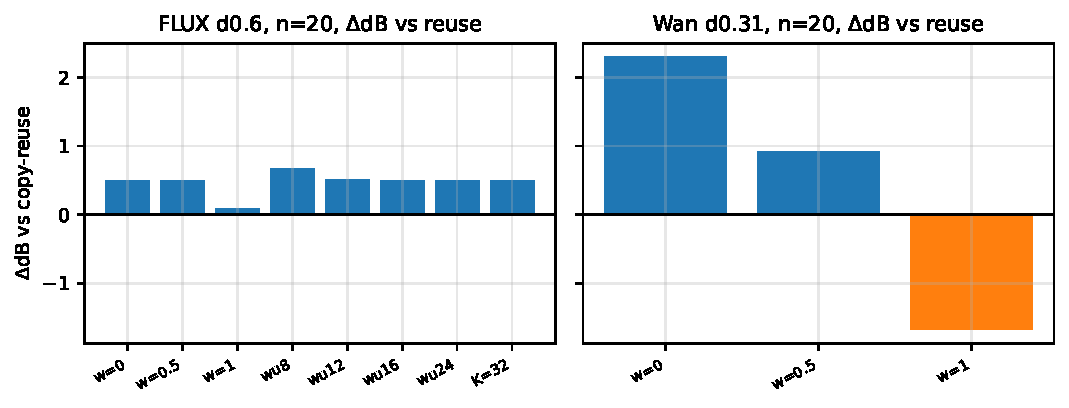
\includegraphics[width=0.9\linewidth]{figs/fig_ablation.pdf}
  \caption{Ablations ($\Delta$dB against copy-reuse, paired on one
  shared base run per panel). Left: FLUX $\delta{=}0.6$, $n{=}20$.
  Right: Wan $\delta{=}0.31$, $n{=}20$. Pure Taylor dominates on Wan
  while the blend remains at or above copy-reuse; pure Chebyshev fails on
  long skip runs; warm-ups of 12 and above never engage the blend; the
  window $K$ has saturated.}
  \label{fig:ablation}
\end{figure}

\section{Additional qualitative results}
\label{app:qual}

\begin{figure}[h]
  \centering
  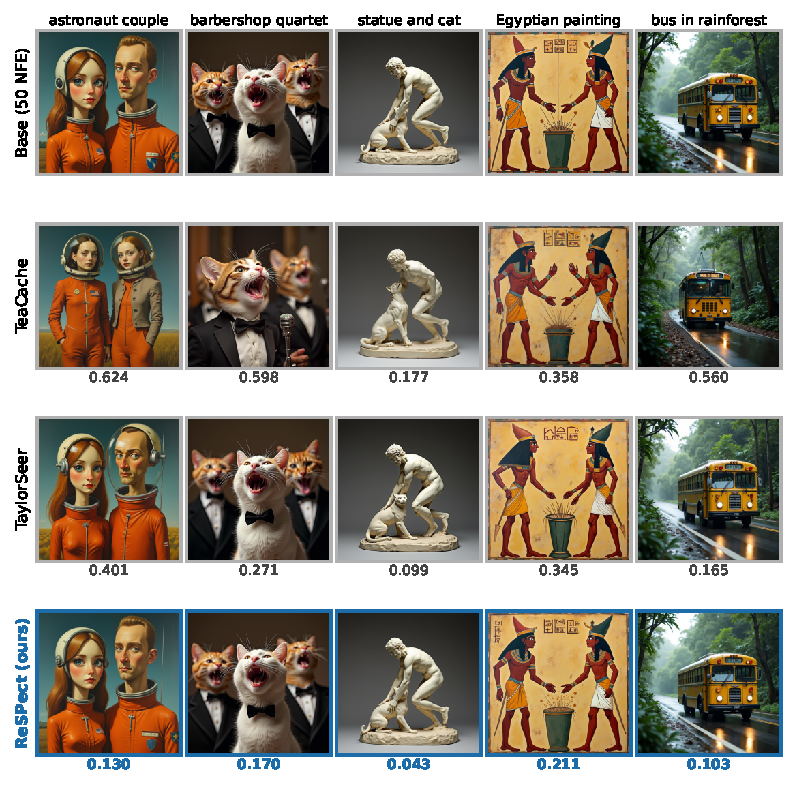
\includegraphics[width=\linewidth]{figs/fig_qual_flux.pdf}
  \caption{FLUX.1-dev at the aggressive budget, all methods run in our
  harness. ReSPect at $\delta{=}0.6$; TaylorSeer ($\mathcal{S}{=}5$) and
  TeaCache ($\delta{=}0.6$) use equal or more compute. LPIPS against the
  base image is printed under each panel. Over 20 DrawBench prompts
  ReSPect attains the lowest LPIPS on 19 (mean $0.183$ vs.\ $0.256$ and
  $0.407$).}
  \label{fig:qual}
\end{figure}

All clips below are generated in our harness on one B200. ReSPect runs
at $\delta{=}0.31$ (Wan, 32 forward passes) and $\delta{=}0.48$
(Hunyuan, 16); TeaCache and TaylorSeer run at their published operating
points and use more compute (Wan 38 and 36, Hunyuan 18 and 18). The two
sentence prompts are (retriever) ``A golden retriever running along a
sandy beach at sunset, waves rolling in behind it'' and (balloon) ``A
red hot air balloon drifting slowly over green rolling hills under a
clear blue sky''; both are also printed in the title of each strip
figure. Per-frame PSNR against the base frame is printed under each
panel. Averaged over all 65 frames, ReSPect leads on every clip:
Wan balloon $34.87$ vs.\ $31.29$ / $17.60$; Wan retriever $30.96$ vs.\
$27.07$ / $17.91$; Hunyuan balloon $37.41$ vs.\ $25.80$ / $21.52$;
Hunyuan retriever $26.04$ vs.\ $16.32$ / $15.24$
(TeaCache / TaylorSeer). The retriever prompt is a difficult motion
case in which all caches degrade while the ordering is preserved.
Tab.~\ref{tab:app-qual} gives the full per-prompt comparison with SSIM
and LPIPS (frame-averaged against the uncached same-seed reference).

\begin{table}[h]
  \centering
  \caption{Per-prompt qualitative-clip comparison: frame-averaged PSNR,
  SSIM, and LPIPS against the uncached same-seed reference over all 65
  frames. NFE is forward passes per clip (Wan base 100, Hunyuan base
  50). ReSPect uses the least compute and leads on every clip and
  metric.}
  \label{tab:app-qual}
  \vspace{0.1cm}
  {\scriptsize\setlength{\tabcolsep}{3pt}
  \begin{tabular}{llcccc}
    \toprule
    Clip & Method & PSNR$\uparrow$ & SSIM$\uparrow$ & LPIPS$\downarrow$ & NFE \\
    \midrule
    Wan retriever & TeaCache & 27.07 & 0.892 & 0.109 & 38 \\
    & TaylorSeer & 17.91 & 0.656 & 0.384 & 36 \\
    & \textbf{ReSPect} & \textbf{30.96} & \textbf{0.937} & \textbf{0.066} & \textbf{32} \\
    \midrule
    Wan balloon & TeaCache & 31.29 & 0.918 & 0.064 & 38 \\
    & TaylorSeer & 17.60 & 0.568 & 0.321 & 36 \\
    & \textbf{ReSPect} & \textbf{34.87} & \textbf{0.950} & \textbf{0.031} & \textbf{32} \\
    \midrule
    Hunyuan retriever & TeaCache & 16.32 & 0.669 & 0.322 & 18 \\
    & TaylorSeer & 15.24 & 0.643 & 0.379 & 18 \\
    & \textbf{ReSPect} & \textbf{26.04} & \textbf{0.878} & \textbf{0.089} & \textbf{16} \\
    \midrule
    Hunyuan balloon & TeaCache & 25.80 & 0.914 & 0.046 & 18 \\
    & TaylorSeer & 21.52 & 0.903 & 0.117 & 18 \\
    & \textbf{ReSPect} & \textbf{37.41} & \textbf{0.980} & \textbf{0.005} & \textbf{16} \\
    \bottomrule
  \end{tabular}}
\end{table}

\begin{figure}[h]
  \centering
  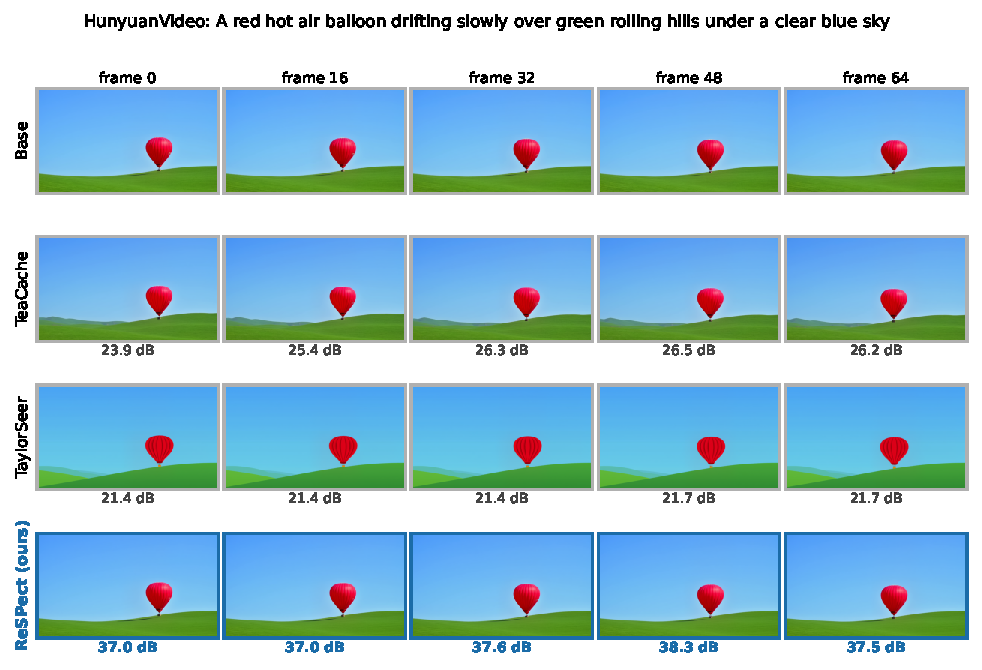
\includegraphics[width=\linewidth]{figs/fig_seq_hunyuan_p1.pdf}
  \caption{HunyuanVideo, balloon clip, $\delta{=}0.48$ (16 NFE).
  TaylorSeer renders a different scene entirely and retains it for the
  whole clip; averaged over all 65 frames, ReSPect scores $37.41$\,dB
  against $25.80$ (TeaCache) and $21.52$ (TaylorSeer).}
  \label{fig:app-qual-hun1}
\end{figure}

\begin{figure}[h]
  \centering
  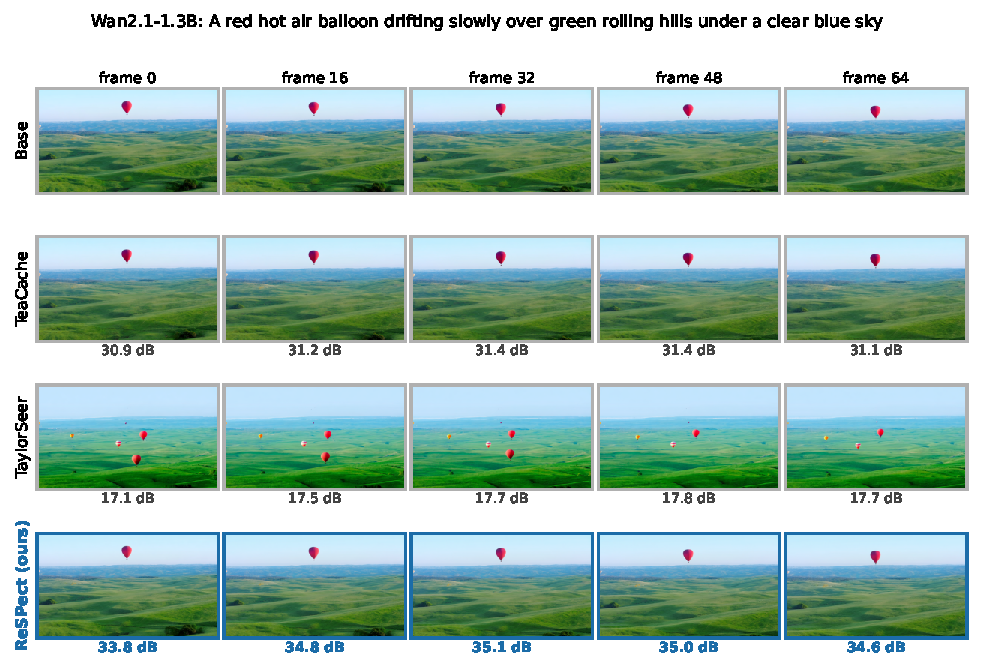
\includegraphics[width=\linewidth]{figs/fig_seq_wan_p1.pdf}
  \caption{Wan2.1, balloon clip, $\delta{=}0.31$ (32 NFE).
  TaylorSeer hallucinates three additional balloons
  and retains them for the whole clip.}
  \label{fig:app-qual}
\end{figure}

\begin{figure}[h]
  \centering
  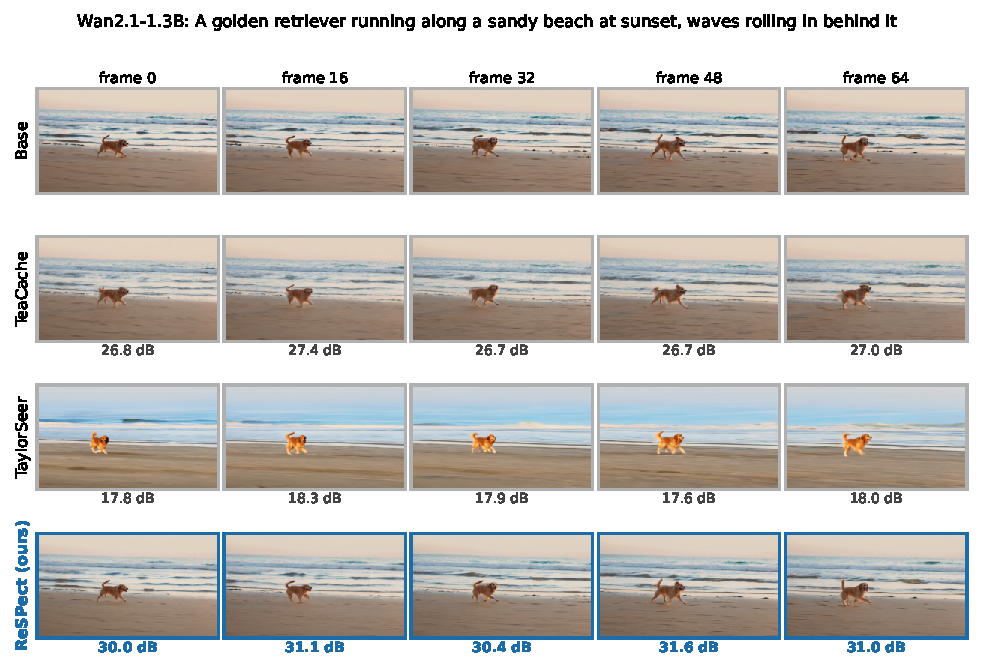
\includegraphics[width=\linewidth]{figs/fig_seq_wan_p0.pdf}
  \caption{Wan2.1, retriever clip, $\delta{=}0.31$ (32 NFE): a difficult
  motion prompt. All methods lie closer to the base here; the forecast
  still gains $+3.9$\,dB over the next baseline, whereas the
  interval-based and raw-distance schedules lose $4$--$13$\,dB.}
  \label{fig:app-qual-wan0}
\end{figure}

\begin{figure}[h]
  \centering
  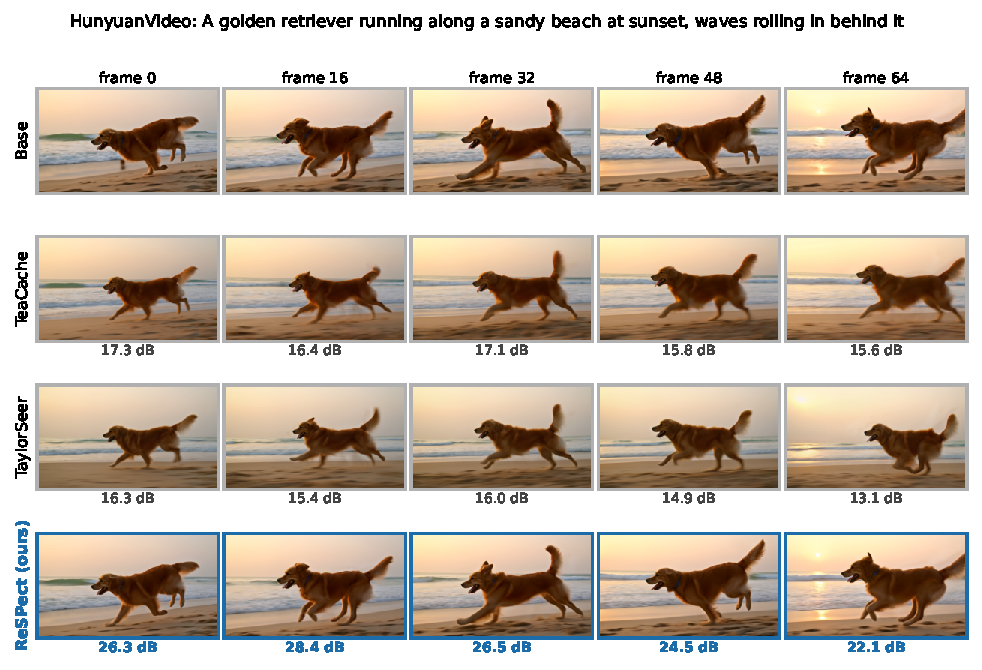
\includegraphics[width=\linewidth]{figs/fig_seq_hunyuan_p0.pdf}
  \caption{HunyuanVideo, retriever clip, $\delta{=}0.48$ (16 NFE).}
  \label{fig:app-qual-hun0}
\end{figure}

